\section{Transportschicht}
\subsection{UDP vs. TCP}
\subsubsection{UDP}
\begin{itemize}
	\item verbindungslos, keine Kontrollmechanismen, bewahrt Reihenfolge nicht
	\item Schnittstelle für einfache Paketvermittlung mittels IP, Verantwortung für Kontrollmechanismen bei Anwendung 
\end{itemize}
\subsubsection{TCP}
\begin{itemize}
	\item verbindungsorientiert, Fehler-, Fluss, Überlastkontrolle, keine Gütegarantie
	\item bietet Abstraktion eines Bytestroms 
\end{itemize}
\subsection{UDP}
\begin{multicols}{2}
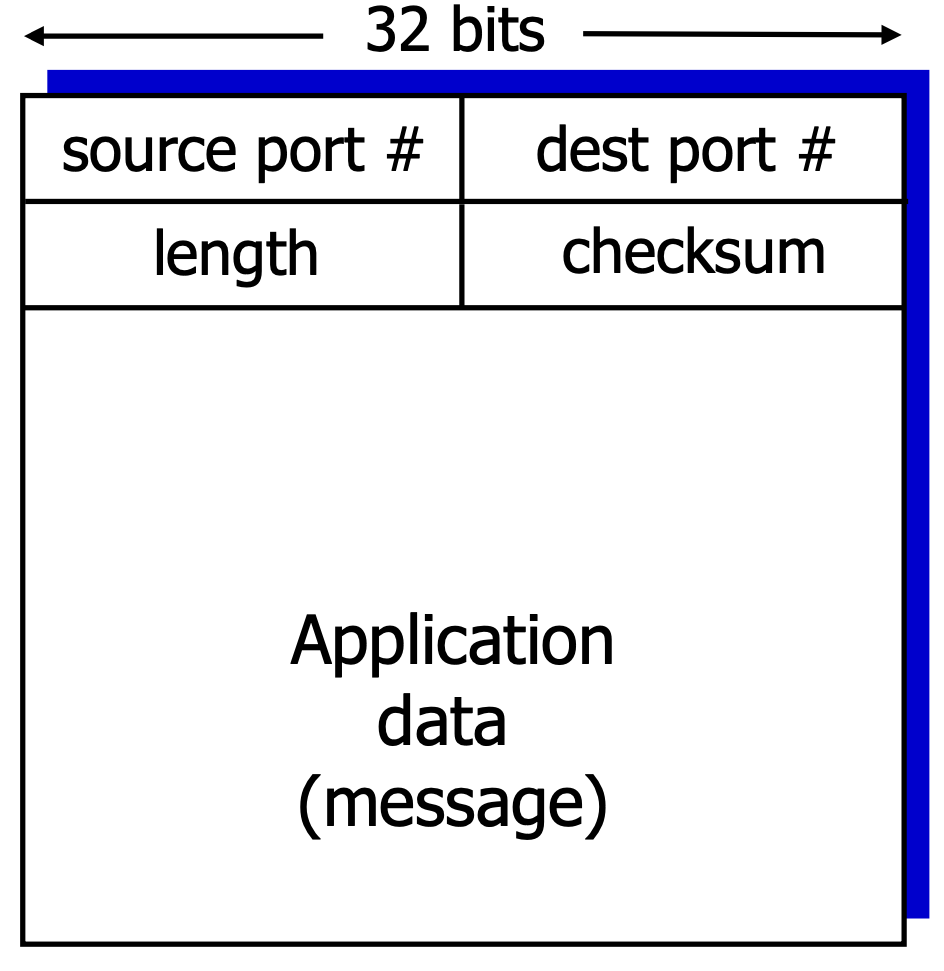
\includegraphics[scale=0.125]{images/UDP_segment.png}
\begin{itemize}
	\item source port: 16 Bit
	\item dest port: 16 Bit
	\item length: 16 Bit (gestates Segment)
	\item checksum: 16 Bit (16 \times 0 \Rightarrow ungenutzt)
\end{itemize}
\end{multicols}
\subsubsection{Multiplexen und Demultiplexen}
\begin{itemize}
	\item Multiplexen: Zusammenführen der Segemente verschiedener Anwendungsprozesse auf Quellhost
	\item Demultiplexen: Ausliefern der Segmente an verschiedene Prozesse des Zielhosts
\end{itemize}
\begin{center}
	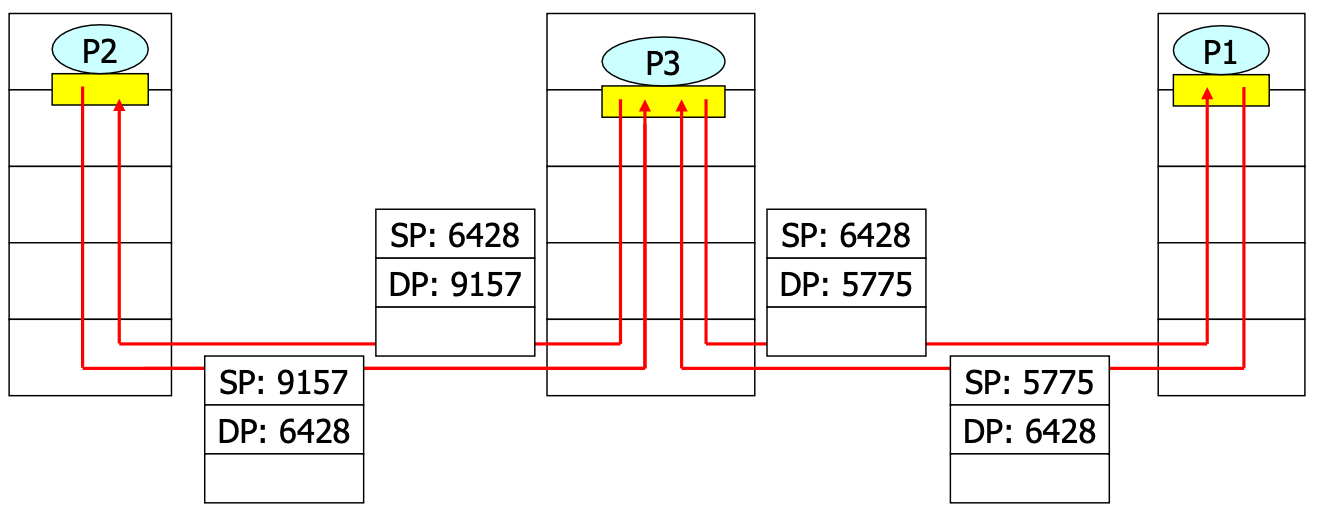
\includegraphics[scale=0.25]{images/UPD_Multiplexen.png}
\end{center}
\subsubsection{Prüfsumme}
\begin{itemize}
	\item Segment wird als Folge von Dualzahlen der Länge 16 Bit aufgefasst
	\item diese werden in Einerkomplementarithmetik addiert
	\item Das Ergebnis wird invertiert und zur Prüfsumme
	\item Empfänger berechnet auch Prüfsumme und addiert diese auf die übergebene \rightarrow $1111111111111111_2$ \Rightarrow kein Fehler liegt vor
	\item Nur einzelne Fehler werden erkannt
\end{itemize}
\subsubsection{Pseudo-header}
\begin{itemize}
	\item Pseudo-header enthält Quell- und Ziel-IP-Adresse, Protokollnummer (17 UDP) und Segmentlänge
	\item UDP des Senders schreibt zuerst 0 ins Checksum-Feld und berechnet dann die Prüfsumme über Segment und Pseudo-header
	\item Vorteil: Es werden fehlgeleitete Pakete erkannt
	\item Nachteil: Verletzung des Schichtenprinzips 
\end{itemize}
\subsection{Fehlerkontrolle}
\begin{center}
	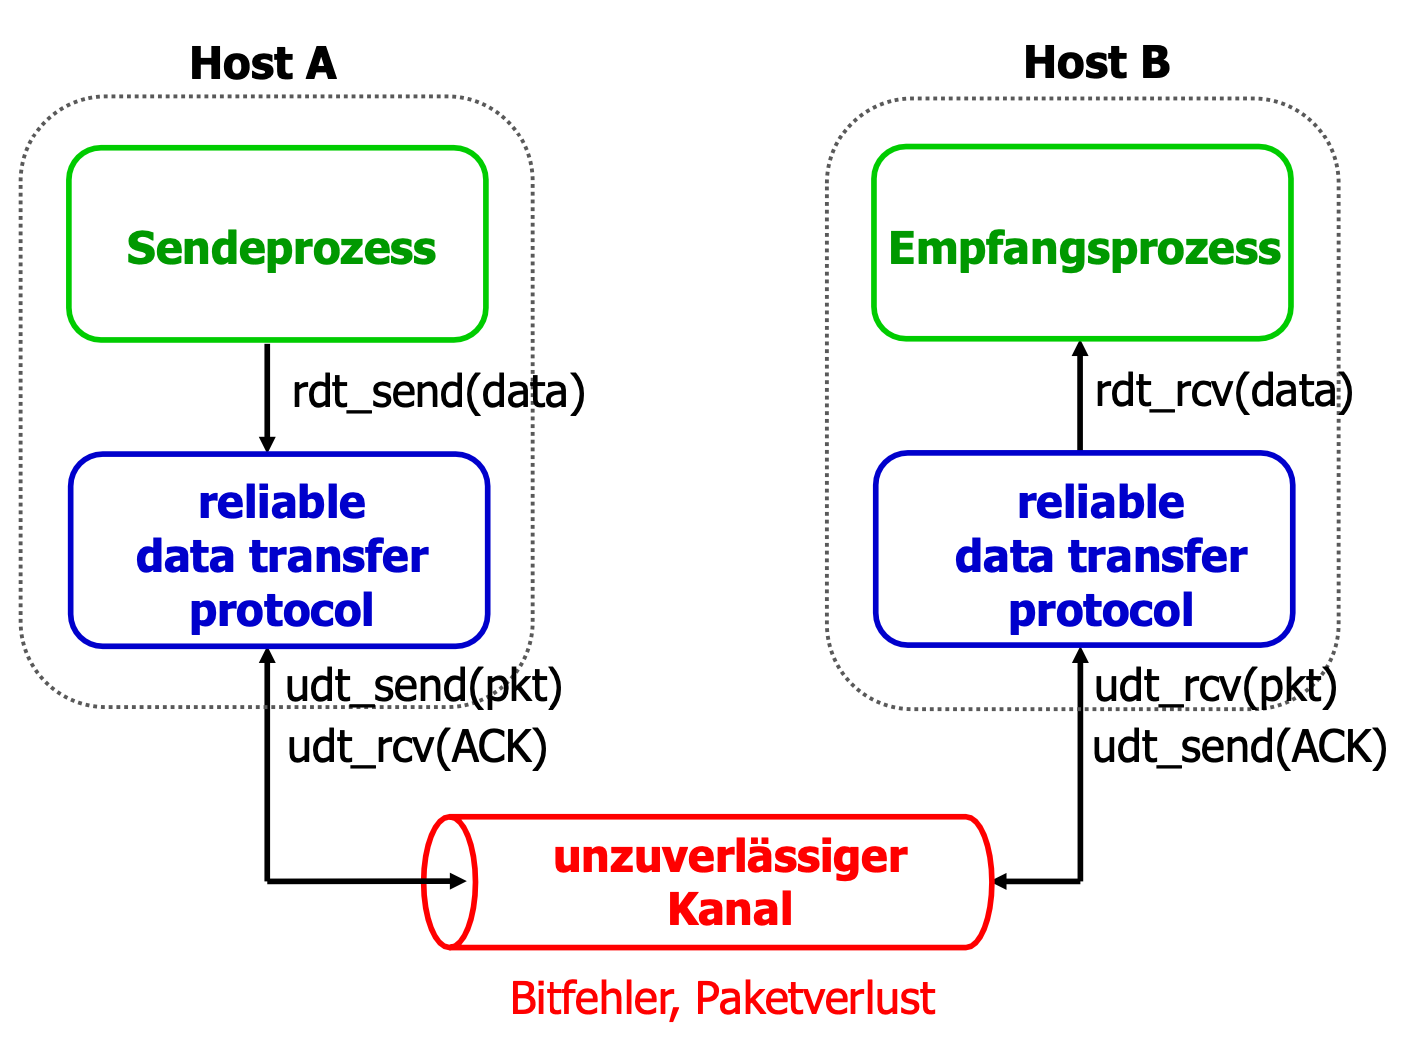
\includegraphics[scale=0.125]{images/Fehlerkontrolle.png}
\end{center}
\subsubsection{Stop-and-Wait}
\begin{multicols}{2}
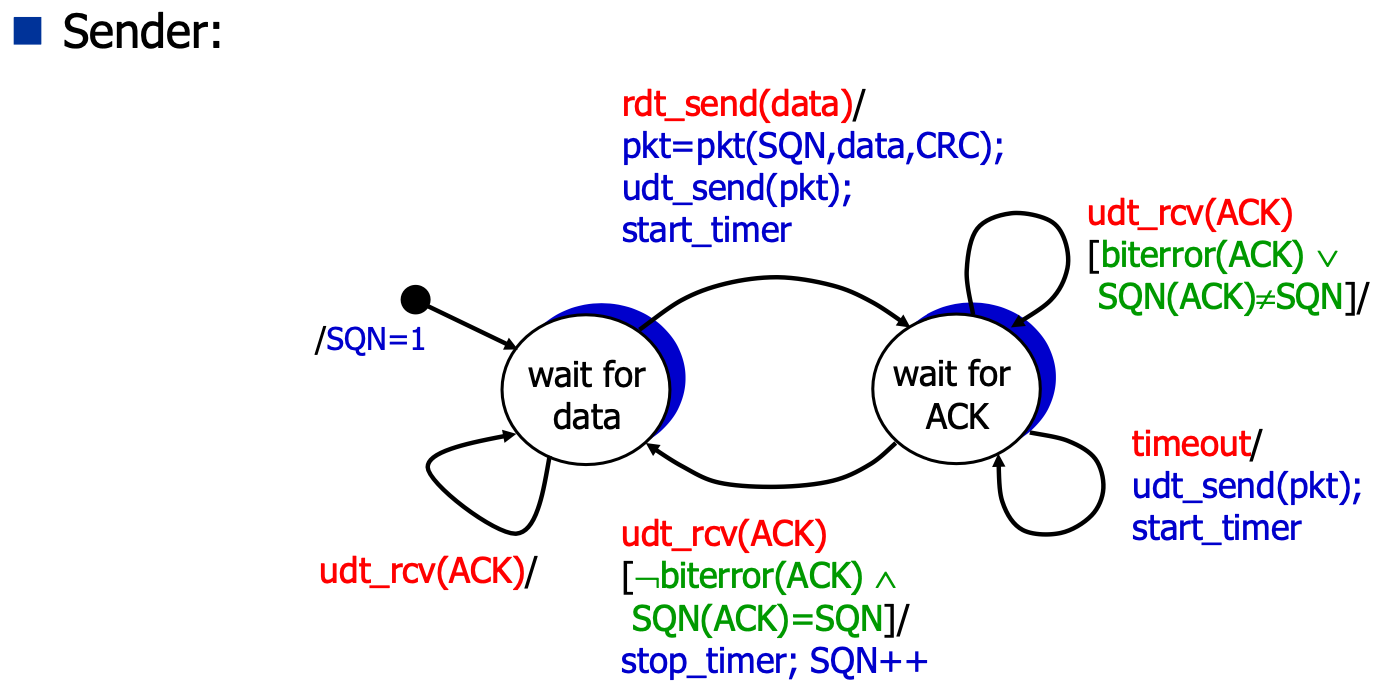
\includegraphics[scale=0.125]{images/Stop_and_Wait_Sender.png}
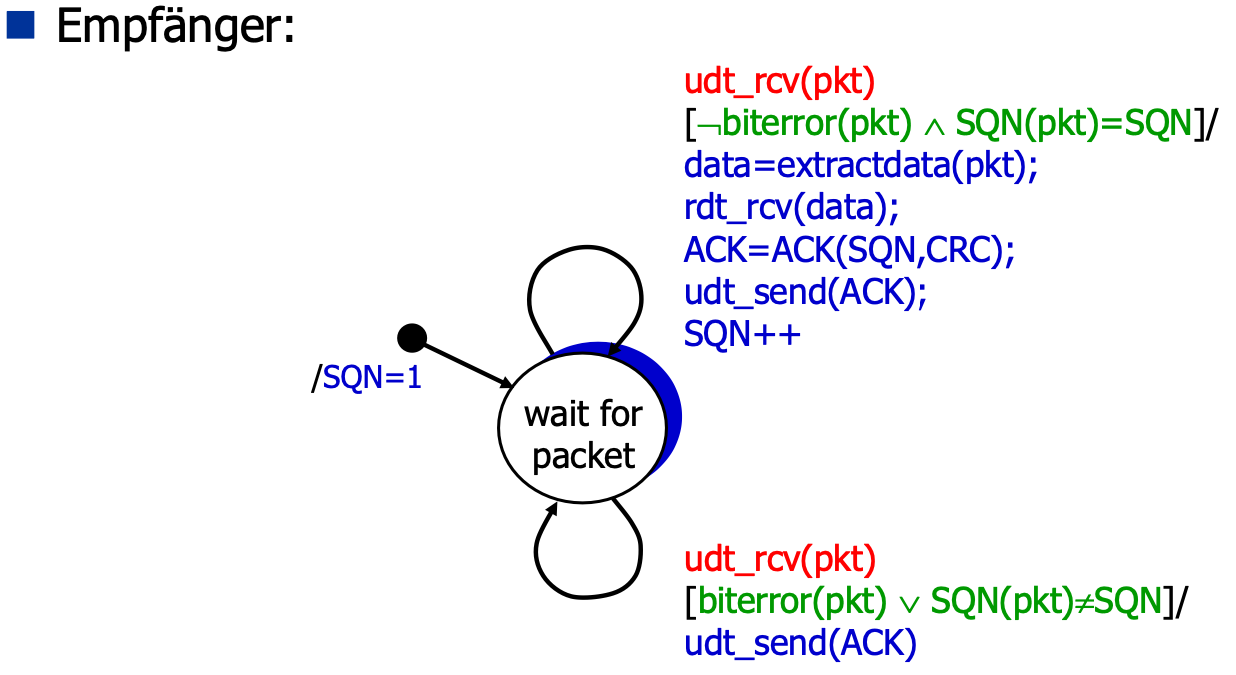
\includegraphics[scale=0.125]{images/Stop_and_Wait_Empfaenger.png}
\end{multicols}
Bei Stop-and-Wait reichen die Sqeuenznummern 0 und 1 \rightarrow Alternating -Bit-Protokoll
\subsubsection{Go-Back-N}
Um die Ineffizienz von Stop-and-Wait zu vermeiden, senden Schiebefensterprotokolle mehrere Pakete, bevor die Bestätigung zurückkommt  
\begin{multicols}{2}
	\begin{itemize}
		\item base: SQN des ältesten unbestätigten Paktes
		\item nextSQN: SQN des nächsten zu verschickenden Pakets
		\item W: Fenstergröße, Anzahl der Pakete, die der Sender vor Erhalt eines ACKs senden darf
	\end{itemize}
	\begin{center}
	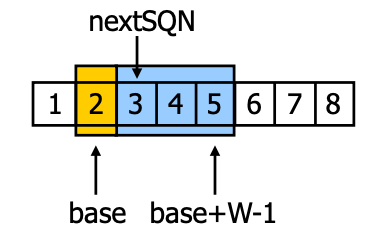
\includegraphics[scale=0.25]{images/Go-Back-N_Sendepuffer.png}		
	\end{center}
\end{multicols}
\begin{multicols}{2}
\begin{center}
	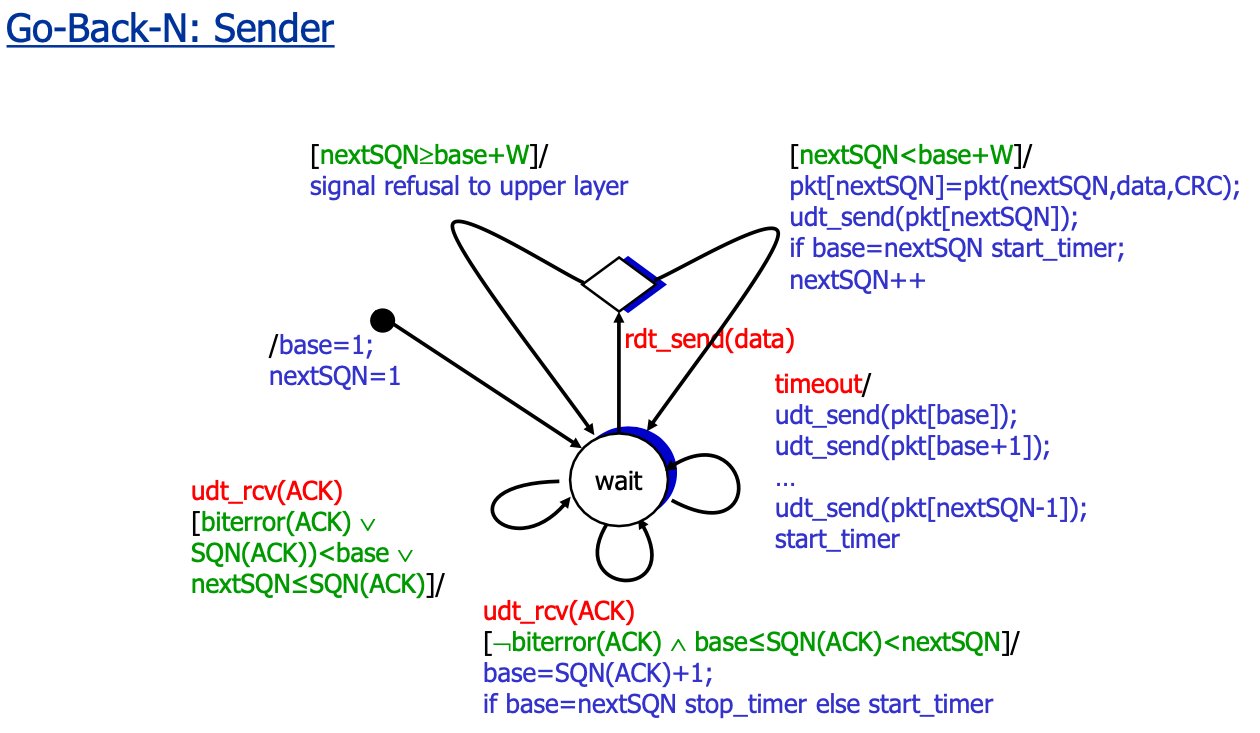
\includegraphics[scale=0.125]{images/Go-Back-N_Sender.png}
\end{center}	
\begin{center}
	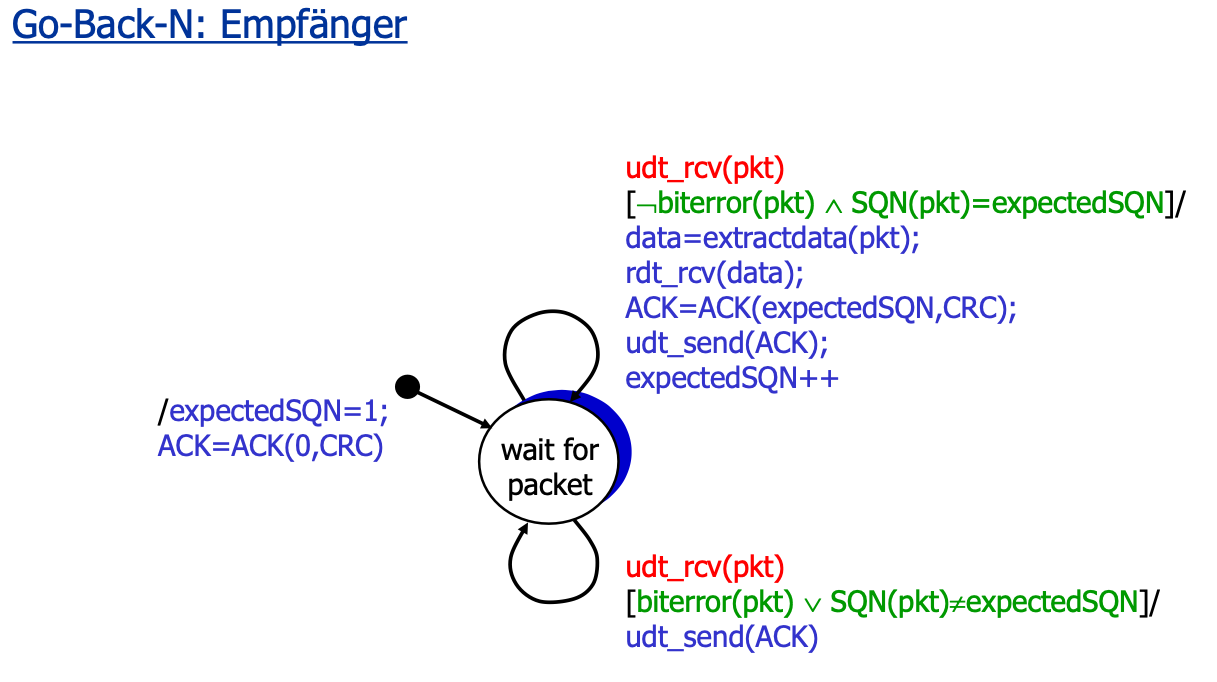
\includegraphics[scale=0.125]{images/Go-Back-N_Empfaenger.png}
\end{center}
\end{multicols}
\subsubsection{Selective Repeat}
\begin{multicols}{2}
\begin{center}
	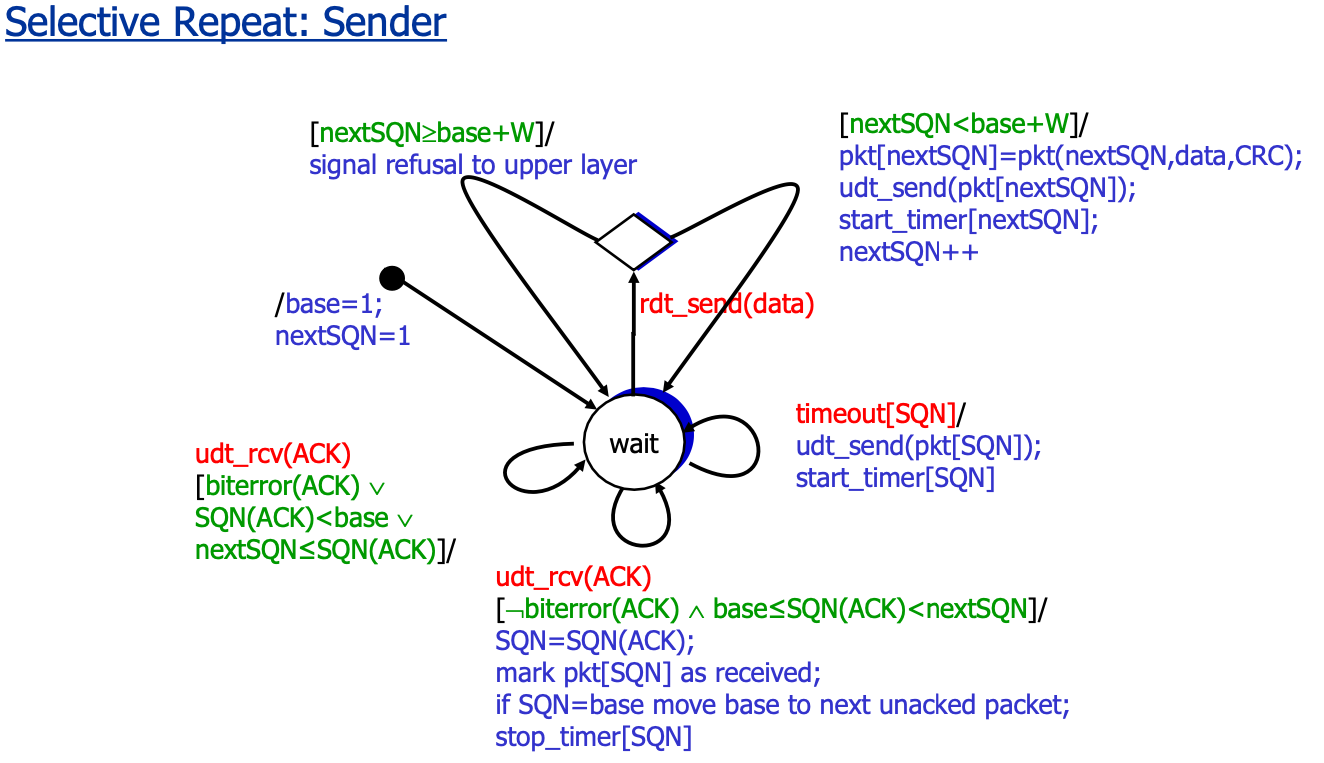
\includegraphics[scale=0.125]{images/Selcetive_Repeat_Sender.png}
\end{center}
\begin{center}
	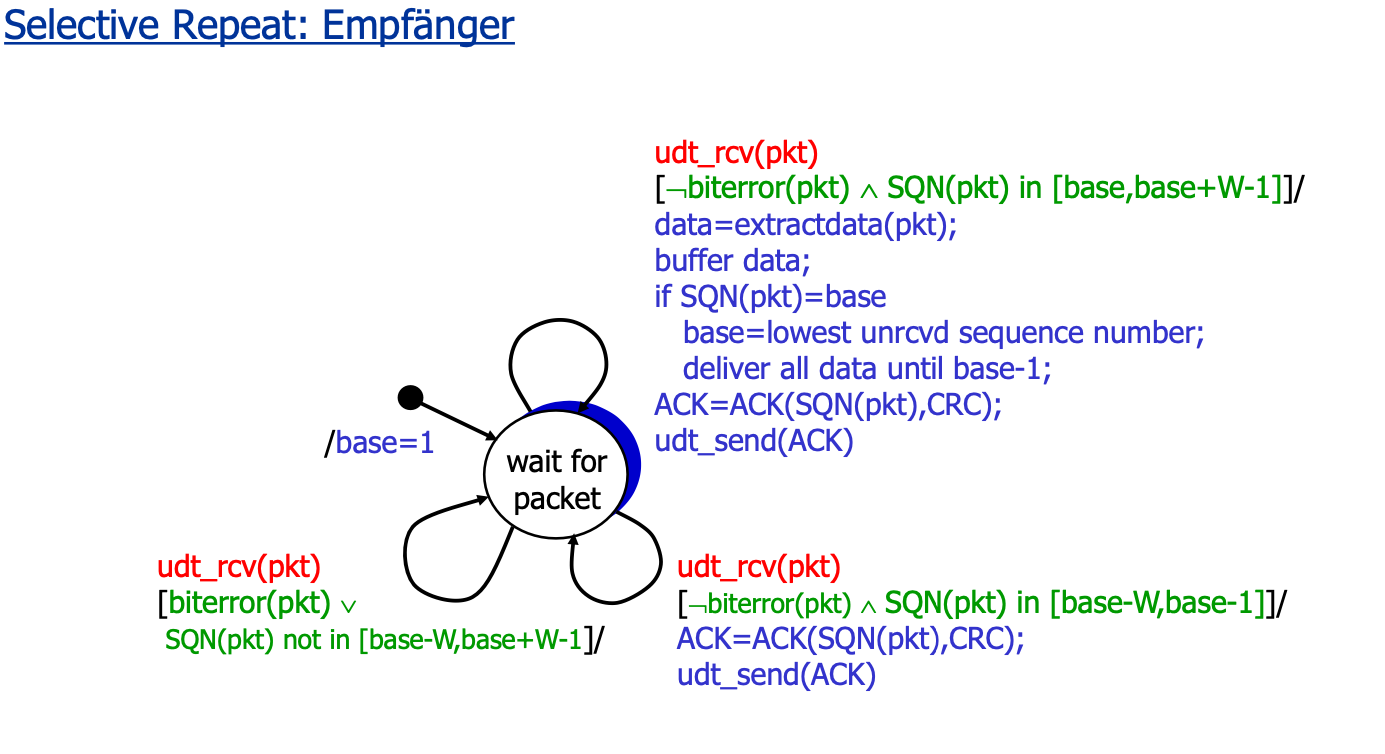
\includegraphics[scale=0.125]{images/Selective_Repeate_Empfaenger.png}
\end{center}
\end{multicols}
\subsubsection{Sequenznummernraum}
Hinreichende Bedingungen: (m Werte, W Fenstergröße)
\begin{itemize}
	\item Empfängerfenstergröße = 1: W < m
	\item Sendefenstergröße = Empfangsfenstergröße = W > 1 : W < (m+1)/2
\end{itemize} 
\subsection{TCP}
\begin{itemize}
	\item Punkt-zu-Punkt
	\item reihenfolgebewahrender Bytestrom
	\item fensterbasierte Fehlerkontrolle
	\item vollduplex: 2 entgegengesetzte Datenströme
	\item verbindungsorientiert
	\item Flusskontrolle
	\item Überlastkontrolle
\end{itemize}
\begin{multicols}{2}
\begin{itemize}
	\item seq: Nummer des ersten Bytes des Segments im Bytestrom
	\item ack: Nummer des nächsten erwarteten Bytes im Bytestrom
	\item Flags:
		\begin{itemize}
			\item CWR (Congestion Window Reduced)
			\item ECE (ECN-Echo)
			\item ACK (ACK gültig)
			\item RST (reset connection)
			\item SYN (synchronisiere Verbindung)
			\item FIN (beende Verbindung)
		\end{itemize}
	\item AdvertizedWindow: Fenstergröße für Flusssteuerung
	\item checksum: wie bei UDP
	\begin{center}
		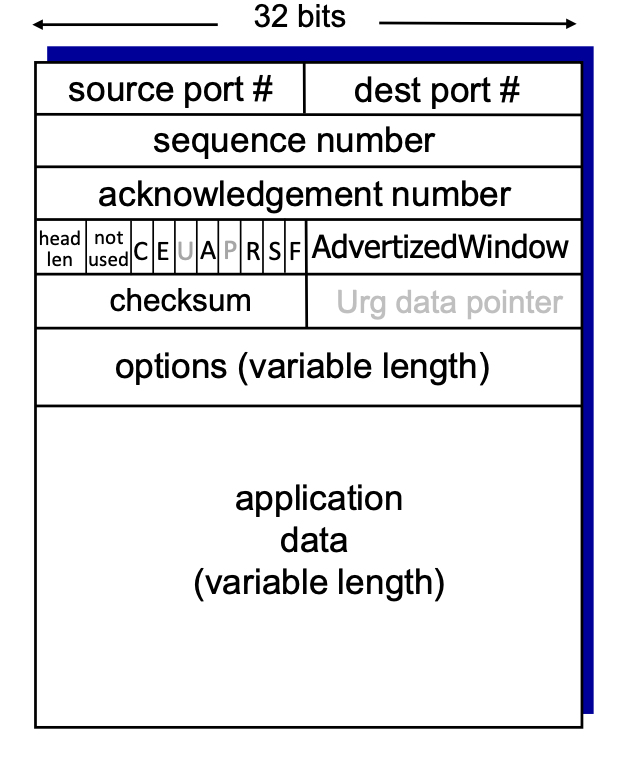
\includegraphics[scale=0.25]{images/TCP_Segment.png}
	\end{center} 
\end{itemize}	
\end{multicols}
\subsubsection{Fehlerkontrolle}
\begin{multicols}{2}
\begin{center}
	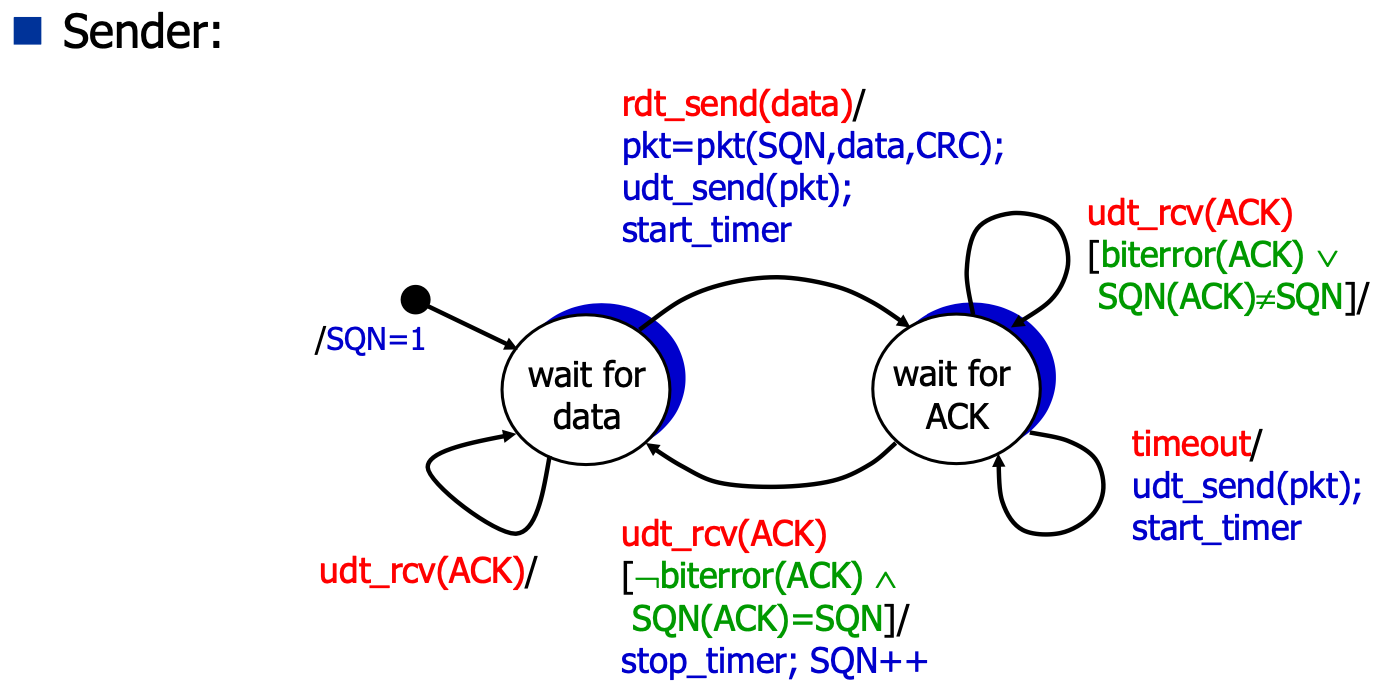
\includegraphics[scale=0.15]{images/Stop_and_Wait_Sender.png}
\end{center}
\begin{center}
	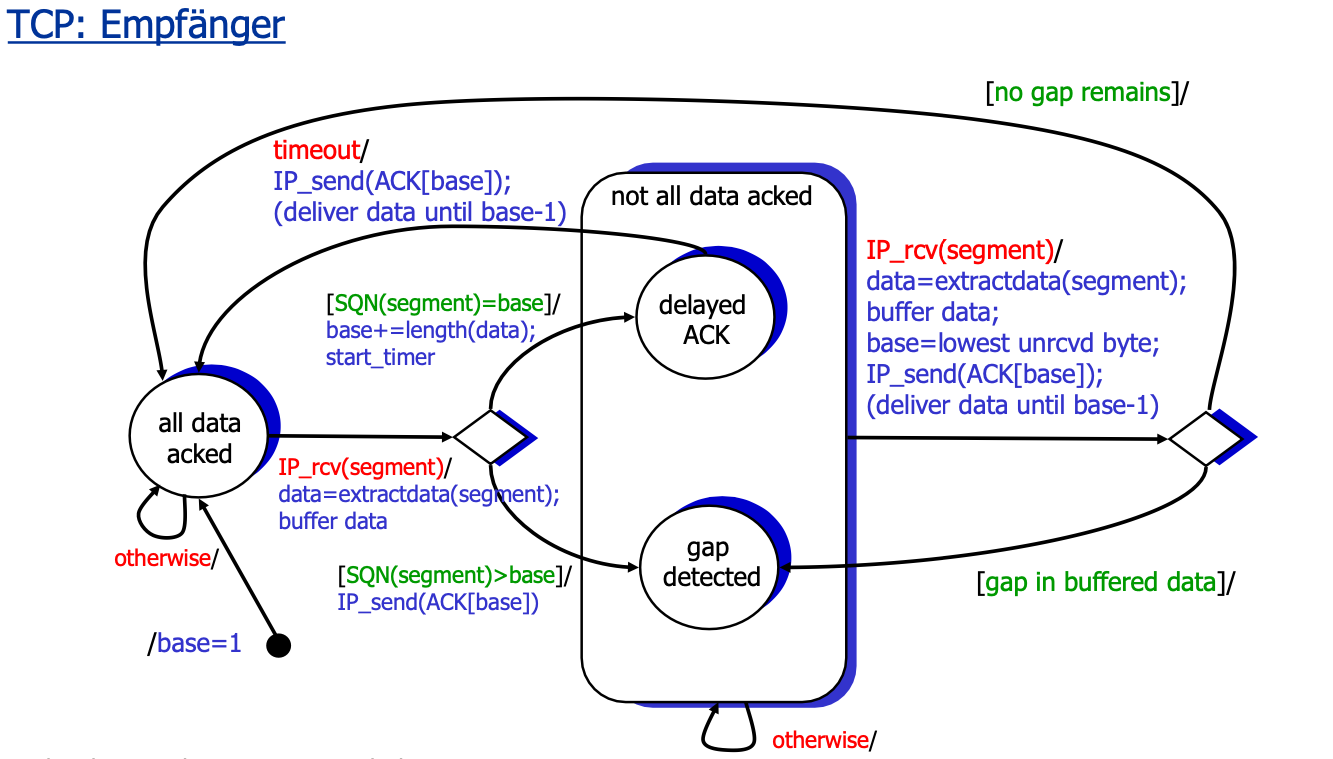
\includegraphics[scale=0.15]{images/TCP_Fehlerkontrolle_Empfaenger.png}	
\end{center}
\end{multicols}
\subsubsection{Verbindungsaufbau}
3-Wege-Handshake:
\begin{enumerate}
	\item SYN-Segment: Client sendet Segment mit SYN-Flag=1, zufälliger initialer Client-SQN (client\_isn), ohne Daten
	\item Server sendet Segment mit SYN-Flag=Ack-Fag=1, zufälliger initialer Srever-SQN (server\_isn), ACK=client\_isn+1, ohne Daten; er legt Puffer und Variablen an
	\item ACK-Segment: Client sendet Segment mit ACK-Flag=1; SQN=client\_isn+1, ACK=server\_isn+1 und ggf. Daten; er elgt Puffer uns Variablen an 
\end{enumerate}
Segmente mit SYN-Flag=1 oder FIN-Flag=1 dürfen keine Daten enthalten
\subsubsection{Verbindungsabbau}
\begin{itemize}
	\item jede Seite kann Verbindungsabbau durch Segment mit FIN-Flag=1 veranlassen
	\item die andere Seite bestätigt mit ACK-Flag=1
	\item beide Seiten müssen ihre Hälfte der Verbindung schließen
	\item hat eine Seite geschlossen, sendet sie keine Daten mehr, nimmt aber noch welche an
	\item Time Wait: die Seite, die den Verbindungsabbruch veranlasst, wartet zum Schluss noch 2 Segmentlebensdauern, um alte Segmente zu empfangen 
\end{itemize}
\subsubsection{Flusskontrolle}
\begin{center}
	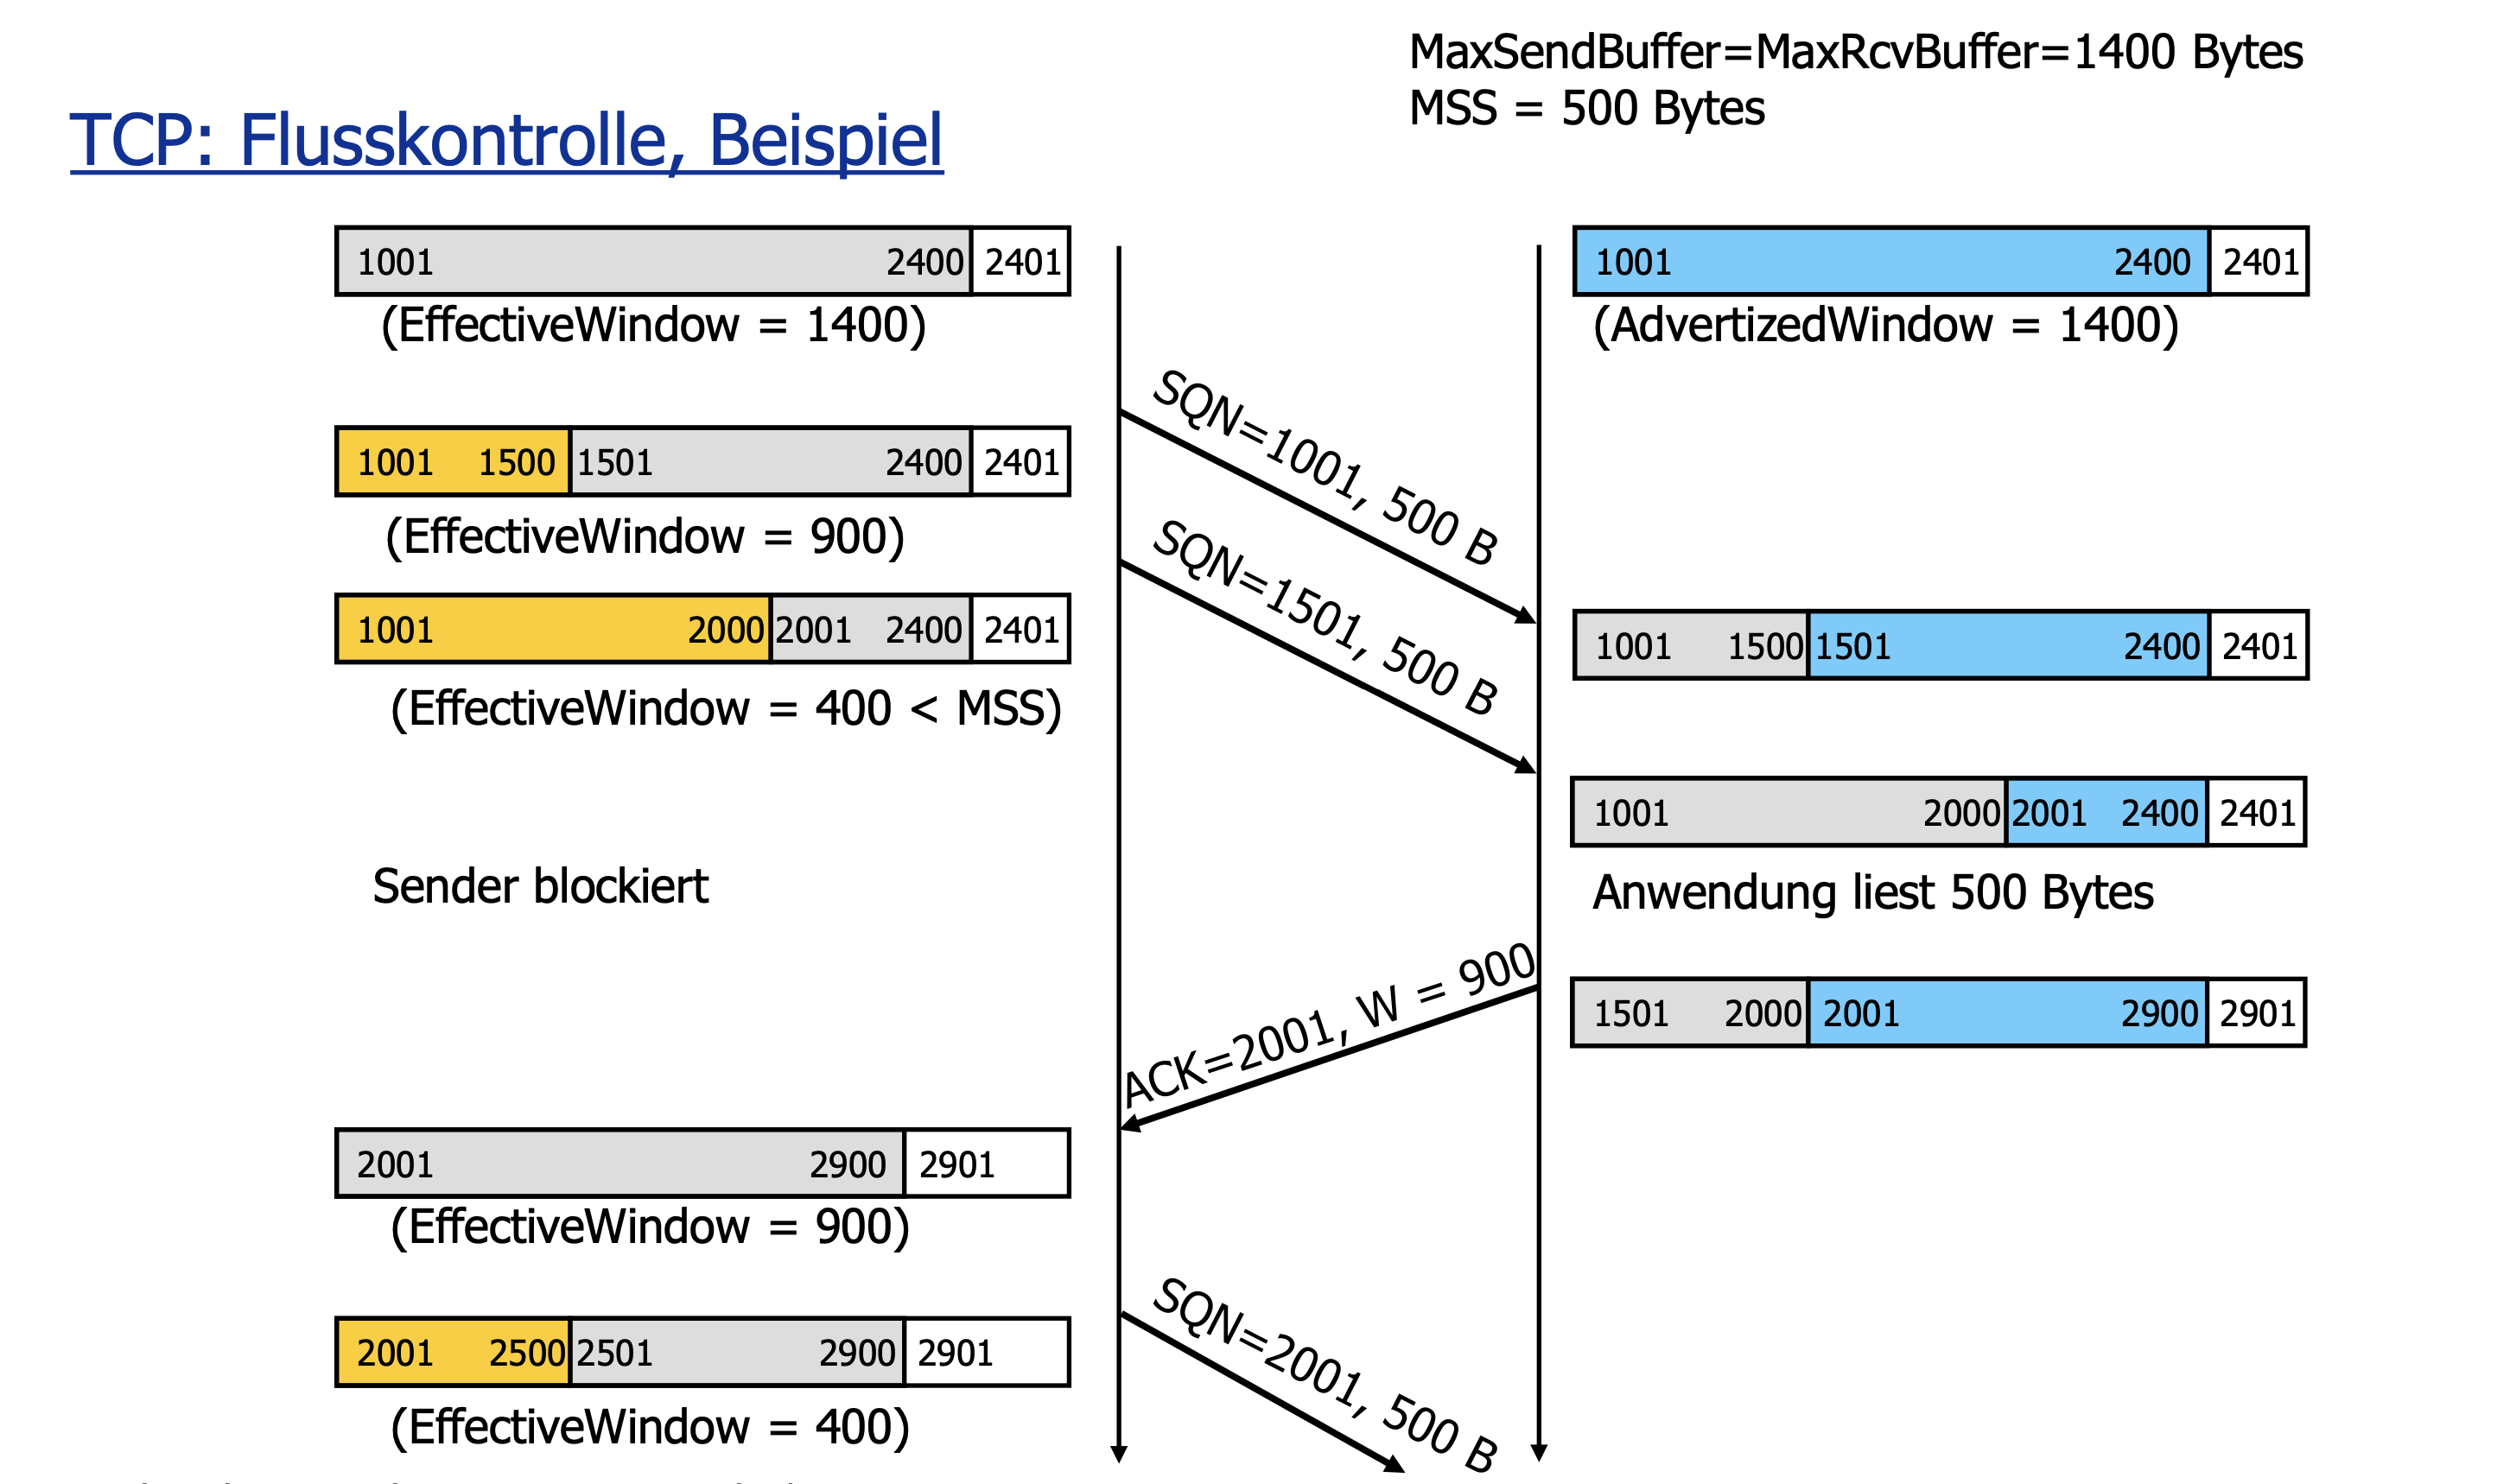
\includegraphics[scale=0.25]{images/TCP_Flusskontrolle.png}
\end{center}
\subsubsection{Überlastkontrolle}
Slow Start:
\begin{enumerate}
	\item CongestionWindow = MSS setzten und bis 3 doppelte ACKs zurückkommen verdoppeln
	\item CongestionWindow wird anschließend halbiert und wächst linear, bis 3 doppelte ACKs zurückkommen (AIMD [Additive Increase, Multiplicative Decrease])
	\item wiederhole AIMD
	\item konservative Reaktion nach Timeout: dann wird Slow Start bis zur hälfte des aktuellen CongestionWindows und danach AIMD durchgeführt
\end{enumerate}





